\documentclass {article}
\usepackage[margin=1.0in]{geometry}
\usepackage[style=mla-new]{biblatex}
\usepackage[hidelinks]{hyperref}
\usepackage{graphicx}
\usepackage{titlesec}
\titlespacing*{\section}{0pt}{3ex plus .5ex minus .2ex}{0ex}
\addbibresource{research.bib}
\newcommand{\sechint}[1]{\small{\emph{#1}} \bigskip}

\begin{document}
\begin{titlepage}
	\centering
	
\includegraphics[width=0.8\textwidth]{images/umd_logo.jpg} \\ \bigskip
	\LARGE{Electrical and Computer Engineering Department \\University of Massachusetts Dartmouth}\\
	\bigskip 
	\LARGE{Master's of Science \\ Thesis Proposal -- Second Draft} \\
	\bigskip 
	\Huge{\bf Investigating Security Credential Management System (SCMS), Vehicular-PKI} \\ \medskip
	\LARGE{\bf By Robert Mushrall III}

	\vfill
	\begin{table}[!hb]
		\centering
		\begin{tabular}{ l l }
			\line(1,0){250} & \line(1,0){150} \\
			\small{Robert Mushrall III}  & \small{Date} \\
			\small{Electrical and Computer Engineering Department} \\
			\small{M.S. Computer Engineering Student} & \\
			\vspace{.3cm} \\
			\line(1,0){250} & \line(1,0){150} \\
			\small{Dr. Hong Liu} & \small{Date} \\
			\small{Electrical and Computer Engineering Department} \\
			\small{Graduate Advisor} & \\
			\vspace{.3cm} \\
			\line(1,0){250} & \line(1,0){150} \\
			\small{Dr. Paul Fortier} & \small{Date} \\
			\small{Electrical and Computer Engineering Department} \\
			\small{Graduate Committee} & \\
			\vspace{.3cm} \\
			\line(1,0){250} & \line(1,0){150} \\
			\small{Brian Hewett} & \small{Date} \\
			\small{Product Manager, General Dynamics Mission Systems} \\
			\small{Graduate Committee} & \\
		\end{tabular}
	\end{table}
	\thispagestyle{empty}
\end{titlepage}
\setcounter{page}{2}

\tableofcontents
\pagebreak

\section{Background}{\sechint{One paragraph (1/3 page) to orient the reader to the area of research.}}

V2V (Vehicle to Vehicle) communications allow vehicles to communicate with each other. A VANET (Vehicular Ad-Hoc NETwork) will open up communication channels, allowing helpful information to be passed between vehicles, alerting drivers of possible hazards or even adjusting routes to minimize travel time. This network will be possible with V2V (Vehicle to Vehicle) and V2I (Vehicle to Infrastructure) communication. V2V communication allows vehicles to pass information, such as speed and nearby dangers, between each other. V2I communication allows vehicles to communicate with an infrastructure that may provide extra benefits to a VANET. SCMS (Secure Credential Management System) aims to combine V2V and V2I to effectively transmit accurate traffic information between vehicles. IEEE Standard 1609.2 defines secure messaging formats for use by WAVE (Wireless Access in Vehicular Environments) devices.

While helpful information can be passed, nodes may act selfishly and not pass information as they should, and malicious information can even be passed instead, causing effects ranging from traffic problems to causing accidents. In order to reduce the effects of misbehaving nodes, communication needs to be secured and the source needs to be verified. SCMS is a V-PKI (Vehicular Public Key Infrastructure) which aims to implement all requirements of CIA (Confidentiality, Integrity, Availability). Confidentiality will be implemented by preserving the privacy of the driver. This will be accomplished by frequently changing certificates. Integrity will be implemented by its design, which includes features to encrypt and sign messages, and manage vehicle certificates. Managing certificates involves issuing certificates to valid vehicles and revoking existing certificates of misbehaving vehicles. Availability can be looked at in a few forms: maintaining low enough overhead to still provide a functional VANET, remain functioning during attacks, and rejecting as few legitimate users as possible.

\section{Problem Statement}{\sechint{One or two sentences that concisely state the problem that will be addressed by the research.}}

As vehicles become more connected and cars become more autonomous, new security risks will begin to show and the effects will become more serious. Currently, there is no standard to effectively secure communication between vehicles. The only applicable standard currently is IEEE 1609.2, which ensures secure messages, not communication. SCMS is a promising V-PKI, and its effectiveness needs to be validated. This thesis will focus on evaluating SCMS in terms of CIA, ensuring that the drivers' privacy is maintained, that messages are valid, and that the system remains available for all valid users.

\section{Technical Discussion}{\sechint{About one page that presents some of the more important aspects of the proposed research. This should include a summary of the state-of-the-art in the particular research area.}}

The nature of VANETs, being wireless with highly dynamic nodes, makes creating an effective means to secure communication especially difficult. Technical challenges, detailed below, mean there is not steady network connection like there is in a traditional network. 

\subsection{Technical Challenges}
Unlike most networks where devices are stationary, devices in a VANET move at high speeds, and in different directions. This dynamic nature means that devices may be neighbors for some distance, or for just a moment \autocite{CommPatterns}. This nature also causes a Doppler shift, requiring the communication devices need to tolerate changes in frequency. The environment itself presents difficulties, such as reflections from buildings or even other vehicles, particularly vehicles that are not part of a VANET. Movement patterns also cause difficulties, especially in routing. Three movement patterns can be defined: city driving, rural roads, and highway \autocite{CommPatterns}.

\subsection{Security Vulnerabilities}
A VANET has potential for security vulnerabilities. The most significant being the possibility of a malicious or malfunctioning vehicle transmitting false data. This poses a concern because it degrades the VANET's purpose of increasing driver (or driverless car) awareness of surroundings. There are many different types of attacks that fall under this issue, ranging from simply injecting bogus information to falsifying a vehicles location to adjust how data is routed to disrupt service \autocite{SecVANet}. Another major vulnerability is privacy. In order to verify data comes from a valid source, the sender needs to be authenticated, however this poses a privacy issue. 

\subsection{Proposed Solutions}
There are several solutions to securing communication while preserving privacy. Reya, et al. suggest several requisites for secure communication. One is security hardware \autocite{SecVeComs}. They recommend a Tamper Proof Device, which will perform all cryptographic operations and storing of cryptographic material. They also recommend an Event Data Recorder, which records critical information which can be used in the event of an accident. Raya, et al. also propose three CRL (Certificate Revocation List) protocols to reduce overhead. The first is called Revocation Protocol of the Tamper-Proof Device, where the CA (Central Authority) sends a message to the Tamper-Proof Device on the revoked vehicle, which then erases all keys. The second, Revocation protocol using Compressed Certificate Revocation Lists, is used when only some of the keys must be revoked. The third, Distributed Revocation Protocol, is used when peers determine that a node is misbehaving and must be revoked. One solution, provided by Carter and Paul, is to use groups combined with public keys \autocite{V_BasedSecOps}. This is a potential solution, however privacy within a group is difficult, and when a member gets revoked, the group key needs to be changed. 

\subsection{The Security Credential Mangement System}
Whyte, Weimerskirch, Kumar and Hehn propose SCMS, the V-PKI that this research will be focused on. This scheme is currently being finalized with the US Department of Transportation \autocite{SecCredMgr}. Figure \ref{scms_overview} represents SCMS as a whole. 
\begin{figure}[!ht]
	\centering
	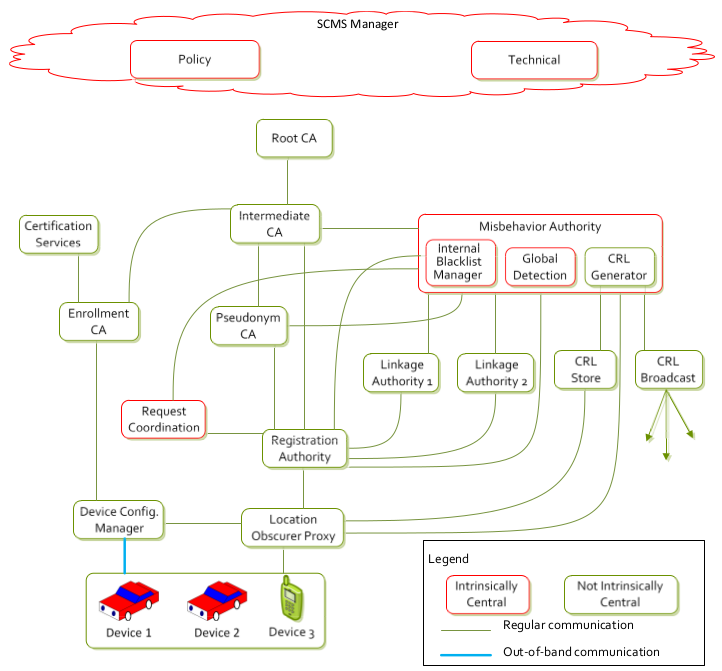
\includegraphics[width=.8\textwidth]{images/scms_overview.png}
	\caption{SCMS Overview}
	\label{scms_overview}
\end{figure}
For privacy reasons, SCMS uses pseudonym certificates, which are certificates that vehicles use instead of a singular certificate. This helps obfuscate the sender of signed messages. To further protections against privacy, SCMS separates operations so that at least two operations need to be compromized before being able to track an individual vehicle. SCMS does not implement a Tamper Proof Device, like suggested Reya, et al. but this also means that SCMS does not rely on the trustworthiness of each particular vehicle. The authors state that one main challenge to their scheme is efficient certificate revocation while protecting drivers' privacy from attackers on the inside.

\section{Approach}{\sechint{One paragraph (1/3 page) that describes the methods that will be applied in conducting the research.}}

SCMS's effectiveness will be evaluated using simulations. The software that will be used is Veins (version 4.6), OMNet++ (version 5.1-2), and Sumo (version 0.30.0-1). OMNet++ is a network simulator that will be used to simulate the protocol and network stacks. This is where most of the V-PKI under test will be implemented. Veins will be used to simulate cars on a road system. This adds the complexity of moving cars in different directions and adds traffic scenarios. To tie the two together, Sumo will be used.
The programming language used will be C++ since that is the language OMNet++ supports. SCMS will be evaluated on three parts: confidentiality, integrity, and availability. Confidentiality will be gauged on the ability to protect vehicles privacy, both from inside attackers and outside attackers. Integrity will be gauged on the ability to prevent invalid information from being spread using authenticated messages. Since SCMS currently doesn't have misbehavior detection, this metric may assume misbehaving nodes and properly functioning nodes are already known. Availability will be measured by the computational overhead SCMS requires, as well as resilience to attacks.

\pagebreak
\section{Works Cited}
\printbibliography

\pagebreak
\section{Schedule and Milestones}{\sechint{Displays a plan for completion of the project or thesis.}}

\begin{table}[!ht]
	\centering
	\begin{tabular}{l|c}
		Task & Time \\ \hline \hline
		Thesis Proposal Submitted & September 12 2017 \\ \hline
		Open Topic Presentation & Late September 2017 \\ \hline
		Tests defined & October 2017 \\ \hline
		Progress Report and Presentation & December 2017 \\ \hline
		Predefense and Progress Report & February 2018 \\ \hline
		Thesis Defense & April 2018 \\ \hline
		Thesis Paper & April 2018 \\ \hline
	\end{tabular}
	\caption{Timeline}
\end{table}

\end{document}
